%%%%%%%%%%%%%%%%%%%%%%%%%%%%%%%%%%%%%%%%%%%%%%%%%%%%
%%%%%%% Verslag Tinlab Advanced Algoritms %%%%%%%
%%%%%%%%%%%%%%%%%%%%%%%%%%%%%%%%%%%%%%%%%%%%%%%%%%%%

\documentclass{article}
\usepackage{graphicx}
\usepackage[font=small,labelfont=bf]{caption}
\usepackage[dutch]{babel}

\usepackage[a4paper, total={6in, 8in}]{geometry}

%Includes "References" in the table of contents
\usepackage[nottoc]{tocbibind}

% libraries for use of Liveness operator
\usepackage{tikz}
\usetikzlibrary{decorations.pathmorphing}
\usepackage{amssymb}

% \addbibresource{references.bib} %Import the bibliography file

\begin{document}

	\sffamily
	%%%%%%% Front page %%%%%%%
	%%%%%%%%%%%%%%%%%%%%%%%%%%%%%%%%%%%%%%%%%%%%%%%%%%%%
	
	\begin{titlepage}
	
		\centering
		  \vfill
		  {\bfseries\Huge
		    Verslag Tinlab Advanced Algorithms \\
		      \vskip2cm
		    }
		    {\bfseries\Large
		      Thijs Dregmans\\
		    }
		    {
		      \bfseries\normalsize
		      1024272\\
		      \vskip1cm
		      \today\\
		  }    
		  \vfill
		  
\includegraphics[width=4cm]{logohr.png} % also works with logo.pdf
		  \vfill
		  \vfill
	    
	\end{titlepage}
	
	\newpage
	
	%%%%%%% Table of Content %%%%%%%
	%%%%%%%%%%%%%%%%%%%%%%%%%%%%%%%%%%%%%%%%%%%%%%%%%%%%
	
	\tableofcontents
	
	\newpage
	
	%%%%%%% Inleiding %%%%%%%
	%%%%%%%%%%%%%%%%%%%%%%%%%%%%%%%%%%%%%%%%%%%%%%%%%%%%
	
	\section{Inleiding}
	
	Voor de cursus 'Advanced Algorithms' van de opleiding Technische Informatica heb ik het volgende verslag geschreven. Het is een verwerking en samenvatting van de lesstof. Het dient zowel als naslagwerk voor mijzelf, als het aantonen van het behalen van de leerdoelen voor de cursus.
	
	Het Tinlab begon met het behandelen van het probleem van specificeren van requirements. Dit is alle design domeinen een groot probleem. Goede requirements definieren is een hoofdpijn dossier. We hebben naar systemen gekeken door het vier variabelen model. Vervolgens zijn een aantal rampen bekeken om dit model in de praktijk te gebruiken om uitspraken te doen over het falen van systemen.

	[geef een samenvatting van de cursus]
	
	\newpage
	
	%%%%%%% Requirements %%%%%%%
	%%%%%%%%%%%%%%%%%%%%%%%%%%%%%%%%%%%%%%%%%%%%%%%%%%%%
	
	\section{Requirements}
	
		Requirements zijn eisen die gesteld worden aan een systeem.
		
		%%%%%%%%%%%%%%%%%%%%%%%%%%%%%%%%%%%%%%%%%%%%%%%%%%%%
		\subsection{Requirements}
		
		Er zijn veel verschillende soorten requirements. Denk dan bijvoorbeeld aan \cite{Lamsweerde2009Requirements}\relax:

		\begin{itemize}
			\item Security requirements
			\item Reliability requirements
			\item Compliance requirements
			\item Development constraints zoals budget
		\end{itemize}

		In dit Tinlab wordt onderscheid gemaakt tussen twee verschillende requirements:

		\begin{enumerate}
			\item System requirements
			\item Software requirements
		\end{enumerate}

		System requirements doen uitspraken over de wereld en de fenomenen in de wereld - of ze spreken over een doel dat bereikt moet worden. Software requirements doen uitspraken over fenomenen in de machine - of over doelen die de machine moet bereiken.

		Software kan van zichzelf niet communiceren met de buitenwereld. Een systeem communiceert met de buitenwereld middels sensoren en actuatoren.
		
		%%%%%%%%%%%%%%%%%%%%%%%%%%%%%%%%%%%%%%%%%%%%%%%%%%%%
		\subsection{specificaties}
		
		[text]
		
		%%%%%%%%%%%%%%%%%%%%%%%%%%%%%%%%%%%%%%%%%%%%%%%%%%%%
		\subsection{Het vier variabelen model}
		
		Een handige manier om systemen te conceptualiseren is het vier variabelen model. Zie Figuur 1 voor een uitwerking van dit model.
		
		\begin{center}
			\begin{minipage}{0.48\linewidth}
				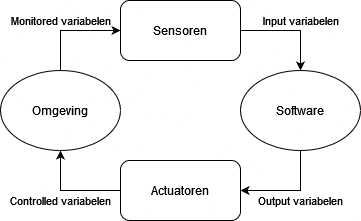
\includegraphics[width=\linewidth]{4variabelen.png}
				\captionof{figure}{4 variabelen model}
			\end{minipage}
			\hfill
		\end{center}

		Dit model komt vooruit het idee van twee werelden die overlappen. Er is een tastbare wereld, met verschillende fenomenen. Deze wereld is de werld waarin wij leven. In deze wereld zijn problemen die wij willen oplossen met systemen. Zo'n systeem is geen onderdeel van de tastbare wereld. Het systeem is een wereld op zichzelf. Er wel enig overlap tussen de syteem-wereld en de tastbare wereld. Het overlap tussen deze werelden is de hardware, specifiek de sensoren en actuatoren.

		De systeem-wereld is de software. Deze wereld heeft in zichzelf geen enkel idee van het bestaan van een ander wereld. De tastbare wereld is de omgeving waarin de het systeem functioneert (of moet functioneren). Ook deze wereld heeft geen idee van de werking van de ander. Dit is ook niet mogelijk of belangrijk, zolang de sensoren en actuatoren naar behoren functioneren.

		De 4 verschillende delen van de van de werelden - omgeving, sensoren, software en actuatoren - communiceren met elkaar met behulp van variabelen.
	
		System requirements definiëren de relaties tussen de monitored variabelen en de controlled variabelen:

		\[ SysReq \subseteq M \times C\]

		Software requirements definiëren de relaties tussen de input variabelen en de output variabelen:


		\[ SoftReq \subseteq I \times O \]
		
			%%%%%%%%%%%%%%%%%%%%%%%%%%%%%%%%%%%%%%%%%%%%%%%%%%%%
			\subsubsection{Monitored variabelen}
			
			Monitored variabelen zijn de variabelen uit de wereld die door de sensoren wordt waargenomen en gemeten.
			
			Ter voorbeeld, een Monitored variabele kan de temperatuur zijn. De omgeving is bijvoorbeeld binnenshuis, bij iemand thuis. De sensor is een temperatuursensor. De sensor meet de waarde/variabele.
			
			%%%%%%%%%%%%%%%%%%%%%%%%%%%%%%%%%%%%%%%%%%%%%%%%%%%%
			\subsubsection{Input variabelen}
			
			Input variabelen zijn de variabelen die door de sensor worden doorgegeven aan de software.

			In het voorbeeld van de temperatuursensor, heeft de temperatuursensor de Monitored variabele omgezet in een reeks bits. Deze bits worden door de sensor naar de microcontroller gestuurd. Voor de software die op de microcontroller staat, is dit de input. In het syteem geldt deze bits als Input variabele.
			
			%%%%%%%%%%%%%%%%%%%%%%%%%%%%%%%%%%%%%%%%%%%%%%%%%%%%
			\subsubsection{Output variabelen}
			
			Output variabelen zijn de variabelen die door de software worden geproduceerd en worden doorgegeven aan de actuatoren.

			In het voorbeeld, heeft de software van de microcontroller de temperatuur - in de vorm van een aantal bits - omgezet in een output. De output is in dit voorbeeld een instructie voor een warmte element om aan te gaan, indien de temperatuur onder een bepaalde waarde zakt. De instructie voor het warmte element is de output van de software, en daarom - in dit voorbeeld - de Output variabele.

			%%%%%%%%%%%%%%%%%%%%%%%%%%%%%%%%%%%%%%%%%%%%%%%%%%%%
			\subsubsection{Controlled variabelen}

			Controlled variabelen zijn de variabelen in de omgeving die door de actuatoren worden beïnvloed, of 'Controlled'.

			In dit voorbeeld, is er door de microcontroller een instructie gegeven aan het warmte element. De microcontroller bevat de software en het warmte element is de actuator. Door de instructie van de software gaat het warmte element aan, en wordt het warmer in huis. De temperatuur stijgt. De Controlled variabele in dit voorbeeld is de temperatuur.

			
			In dit voorbeeld is de Controlled variabele en de Monitored variabele dezelfde variabele, maar dat hoeft niet zo te zijn. Men kan in plaats van een warmte element, ook een lampje aansluiten, die dan aan zou gaan bij een bepaalde temperatuur. In dit geval zou de Controlled variabele het licht van het lampje zijn.
		
		%%%%%%%%%%%%%%%%%%%%%%%%%%%%%%%%%%%%%%%%%%%%%%%%%%%%
		\subsection{Rampen}
		
		De werking van het vier variabelen model wordt gedemonstreerd aan de hand van een aantal rampen.
		
			%%%%%%%%%%%%%%%%%%%%%%%%%%%%%%%%%%%%%%%%%%%%%%%%%%%%
			\subsubsection{Therac-25}
			\begin{description}
				\item[Beschrijving] 
				In de Verenigde Staten vonden in de jaren 80 een serie ongelukken plaats, waarbij verschillende patienten een dodelijke dosis straling kreeg toegediend met de Therac-25. Anderen raakten zwaar-gewond. \cite{274940}\relax De Therac-25 verschilde met zijn voorloper - de Therac-20 - op een belangrijke manier. De Therac-20 is ook een computergestuurde machine, maar heeft ook hardware veiligheidsmaatregelen. In de Therac-25 zijn deze hardware veiligheidsmaatregelen verdwenen en vervangen door software die hetzelfde effect zouden moeten hebben. \cite{thomas1994story}\relax
				\item[Datum en plaats] 
				De ongelukken vonden plaats in de Verenigde Staten, tussen 1985 en 1987 \cite{274940}\relax.
				\item[Oorzaak]
				De zes ongelukken is aan verschillende zaken te wijden:
				\begin{itemize}
					\item De Therac-25 verwijderde de veiligheidshardware die wel aanwezig was op de Therac-20.
					\item De Therac-25 had cryptisch foutmelding, die vaak enkel het woord "malfunction" bevatten, samen met een error code - een getal van 1 tot 64. Het was voor de gebruiker onduidelijk wat deze betekenden. Het was niet duidelijk of een dergelijke foutmelding de patient in gevaar kon brengen. Ook in de handleiding wordt niet gesproken over foutcodes.
					\item De Therac-25 heeft 3 modi. Door een meganisch-draaiende schijf werd de installatie gereed gemaakt voor de juiste modus. Een sensor detecteerde of de schijf in de juiste positie stond. Deze gaf een 3 bits waarde terug. Een kleine foute elektronische fout kan een incorrect waarde teruggeven, waardoor een patient een overdosis kan krijgen.
					\item De installatie gereed maken kost 8 seconden. Als de gebruiker kiest voor een bepaalde opstelling, dan wordt die gereed gemaakt. Als de gebruiker dan vervolgens nog voordat de installatie gereed is, de opstelling wijzigt, dan wordt dit niet opgemerkt. Op het scherm wordt de juiste opstelling getoond, maar in werkelijkheid is het systeem nog niet gereed.
				\end{itemize}
				
			\end{description}
			
			%%%%%%%%%%%%%%%%%%%%%%%%%%%%%%%%%%%%%%%%%%%%%%%%%%%%
			\subsubsection{Vlucht 1951}
			\begin{description}
				\item[Beschrijving]
				
				\item[Datum en plaats] 
				
				\item[Oorzaak]
				
			\end{description}
			
			%%%%%%%%%%%%%%%%%%%%%%%%%%%%%%%%%%%%%%%%%%%%%%%%%%%%
			\subsubsection{Tsjernobyl}
			\begin{description}
				\item[Beschrijving]
				
				\item[Datum en plaats] 
				
				\item[Oorzaak]
				
			\end{description}
			
			%%%%%%%%%%%%%%%%%%%%%%%%%%%%%%%%%%%%%%%%%%%%%%%%%%%%
			\subsubsection{Self-driving cars}
			\begin{description}
				\item[Beschrijving] 
				
				\item[Datum en plaats] 
				
				\item[Oorzaak]
				
			\end{description}
			
			%%%%%%%%%%%%%%%%%%%%%%%%%%%%%%%%%%%%%%%%%%%%%%%%%%%%
			\subsubsection{Stints},
			\begin{description}
				\item[Beschrijving] 
				
				\item[Datum en plaats] 
				
				\item[Oorzaak]
				
			\end{description}
			
			%%%%%%%%%%%%%%%%%%%%%%%%%%%%%%%%%%%%%%%%%%%%%%%%%%%%
			\subsubsection{Radiologische ongelukken in Bialystok, Polen}
			\begin{description}
				\item[Beschrijving] 
				
				\item[Datum en plaats] 
				
				\item[Oorzaak]
				
			\end{description}
			
		
	\newpage
	
	%%%%%%% Modellen %%%%%%%
	%%%%%%%%%%%%%%%%%%%%%%%%%%%%%%%%%%%%%%%%%%%%%%%%%%%%
	
	\section{Modellen}
	
	Om systemen efficïent en waarheidsgetrouw te kunnen modelleren gebruiken we State Transition Diagrams. In deze diagrammen worden de zogenoemde 'states' als punten afgebeeld. In een systeem kunnen tussen deze states geswitcht worden. Dit noemen we transities.

	[voeg voorbeeld van STD in]

	Er zijn veel verschillende soorten diagrammen. Dit TINLAB focust op Kripke structuren.
	
		%%%%%%%%%%%%%%%%%%%%%%%%%%%%%%%%%%%%%%%%%%%%%%%%%%%%
		\subsection{De Kripke structuur}
		
		Een state is een beschrijving waarin een systeem zich gedurende een tijd bevindt.

		[voeg voorbeeld van Kripke structuur in]

		Laten we als voorbeeld een stoplicht nemen. Men zou kunnen zeggen dat er in dit systeem vier verschillende states zijn:

		\begin{itemize}
			\item Rood licht
			\item Oranje licht
			\item Groen licht
			\item Oranje knipperend licht (error state)
		\end{itemize}

		Een systeem heeft altijd een begintoestand. Dit wordt de 'initial state' genoemd. Dit is de toestand waarmee het systeem start. 
		x = 0

		We noemen de verzameling van alle states 'S'. Elke individuele state noemen we s0, s1, s2 en s3.

		s0...s3 e S

		Tussen deze vier toestanden zijn verschillende transities mogelijk. Alle transitiesrelaties die mogelijk zijn:

		S = {s0, s1, s2, s3}
		R ? S x S = {
			(s0, s0), (s0, s1), (s0, s2), (s0, s3),
			(s1, s0), (s1, s1), (s1, s2), (s1, s3),
			(s2, s0), (s2, s1), (s2, s2), (s2, s3),
			(s3, s0), (s3, s1), (s3, s2), (s3, s3),
		}

		Niet al deze transitie relaties zijn logisch en komen in de werkelijkheid voor. Zo is bijvoorbeeld de transitierelatie van Rood licht naar Oranje licht niet gebruikelijk.
		
		Alle systemen die wij modelleren zijn reactief. Dat betekent dat elke state een uitgaande transitierelatie moet hebben. Dit wordt ook wel een 'totaal' systeem genoemd.
		
		%%%%%%%%%%%%%%%%%%%%%%%%%%%%%%%%%%%%%%%%%%%%%%%%%%%%
		\subsection{Tijd}
		
		
		
		%%%%%%%%%%%%%%%%%%%%%%%%%%%%%%%%%%%%%%%%%%%%%%%%%%%%
		\subsection{Guards en Invarianten}
		
		In de tool Uppaal kunnen we met Kripke structuren systemen modelleren. Elke toestand kan Invarianten krijgen. Elke transitierelatie kan Guards krijgen.
		
		Met een Invariant kunnen we eisen dat een bepaalde stelling altijd waar moet zijn zolang het systeem in die toestand is. Als de stelling niet meer waar is, dan wordt een transitie geforceerd.

		Met een Guard kunnen we eisen dat een bepaalde transitie alleen genomen kan worden als een bepaalde stelling waar is.
		
		%%%%%%%%%%%%%%%%%%%%%%%%%%%%%%%%%%%%%%%%%%%%%%%%%%%%
		\subsection{Deadlock}
		
		Een deadlock wordt veroorzaakt door een combinatie van Guards en Invarianten waardoor tijd niet kan verstrijken.

		In Uppaal is tijd een continu verschijnsel. Alle klokken lopen even snel. Tijd kan alleen verstrijken in states. Het kost dus exact 0 tijd om een transitie te nemen. Als de Guards en Invarianten op een bepaalde manier zijn ingesteld, dan kan het zo zijn dat tijd niet kan verstrijken in het model. Dit heet een 'deadlock'.
		
		%%%%%%%%%%%%%%%%%%%%%%%%%%%%%%%%%%%%%%%%%%%%%%%%%%%%
		\subsection{Zeno gedrag}
		
		Zeno gedrag is vernoemd naar de Griekse filosoof Zeno van Elea. Hij is bekend van verschillende paradoxen. Hier gaat het over de race tussen de schildpad en Achilles:
		
		De schildpad gaat een wedstrijd aan met Achilles en zegt tegen hem dat hij zal winnen, zolang hij maar een voorsprong krijgt. De schildpad krijgt een voorsprong en de tijd begint te lopen. De redenering van de schildpad is als volgt: Als Achilles is aangekomen waar de schildpad begon, heeft de schildpad in de tussentijd tijd gehad om verder te komen. Dus Achilles zal de schildpad nooit inhalen. De redenering van de schildpad klopt niet.

		Het probleem is dat in een eindige hoeveelheid tijd er een oneindig aantal handelingen kan worden verricht.


		[ geef meer uitleg]
		
	\newpage
	
	%%%%%%% Logica %%%%%%%
	%%%%%%%%%%%%%%%%%%%%%%%%%%%%%%%%%%%%%%%%%%%%%%%%%%%%
	
	\section{Logica}
	
	'Logica' komt van het Griekse woord 'logos', dat 'woord' en 'argument' betekent. Al duizenden jaren is men bezig met logica. Het wordt ook wel de kunst van formeel redeneren genoemd. Het is onder andere de basis voor de filosofie en wiskunde. Ook in de Informatica gaat het veel over logica.

	Er wordt in de logica onderscheid gemaakt tussen verschillende soorten logica. Het makkelijkste voorbeeld is Syllogisme van Aristoteles. Zo'n redenering gaat volgens 3 stappen:

	\begin{enumerate}
		\item (algemene stelling) Alle mensen hebben een hoofd.
		\item (bijzondere stelling) Thijs is een mens.
		\item (conclusie) Thijs heeft een hoofd.
	\end{enumerate}

	Op deze manier kan een conclusie bewezen worden. Als de eerste twee stelling kloppen, dan klopt de conclusie ook. Daar is niets tegen in te brengen. Dit wordt ook wel deductie genoemd.

	Verder wordt ook onderscheid gemaakt tussen Propositielogica en Predicatenlogica.
	
		%%%%%%%%%%%%%%%%%%%%%%%%%%%%%%%%%%%%%%%%%%%%%%%%%%%%
		\subsection{Propositielogica}
		
		Propositielogica maakt gebruik van Proposities. Proposities zijn uitspraken die waar of niet waar zijn. Voor de notatie worden hier vaak letters voor gebruikt, zoals in de wiskunde. Voorbeelden van Proposities zijn:

		\begin{itemize}
			\item \( 4 > 10 \)
			\item De aarde is plat.
			\item Alle mensen hebben twee handen.
			\item Door 2 punten kan altijd een rechte lijn getrokken worden.
		\end{itemize}

		Naast Proposities zijn er ook stellingen en axioma. Stellingen zijn Proposities die te bewijzen zijn, zoals bijvoorbeeld de stelling van Pythagoras. Tijdens zo'n bewijs moet men aannames doen. Sommige dingen zijn zó fundamenteel dat ze niet te bewijzen zijn. Als men tracht deze te bewijzen kan een cirkelredenering ontstaan. Zo'n fundamentele aanname heet een axioma. Het is een grondslag, waar geen bewijs voor is. bijvoorbeeld:

		\begin{itemize}
			\item 0 is een getal
			\item \( 0 \leq P(A) \leq 1 \), als \( A \subseteq S \)
			\item (Wet van non-contradictie) Een stelling kan niet - op hetzelfde moment, op dezelfde manier - waar en niet waar zijn.
		\end{itemize}
		
		%%%%%%%%%%%%%%%%%%%%%%%%%%%%%%%%%%%%%%%%%%%%%%%%%%%%
		\subsection{Predicatenlogica}
		
		In de logica zijn de Wetten van De Morgan van belang. De Wetten van De Morgan stellen dat twee stellingen met een 'en' operator te schrijven zijn met een 'of' operator met een aantal 'niet' operatoren, en andersom:
	
		\begin{itemize}
			\item \( (p \land q) \equiv \neg(\neg p \lor \neg q) \)
			\item \( (p \lor q) \equiv \neg(\neg p \land \neg q) \)
		\end{itemize}
		
		%%%%%%%%%%%%%%%%%%%%%%%%%%%%%%%%%%%%%%%%%%%%%%%%%%%%
		\subsection{Kwantoren}
		
		Er zijn 2 belangrijke kwantoren:

		\begin{itemize}
			\item De existentiekwantor (\( \exists \))

			Wanneer deze kwantor voor een predikaat staat, betekent dat `voor ten minsten één`.

			\item De universele kwantor (\( \forall \))

			Wanneer deze kwantor voor een predikaat staat, betekent dat `voor alle`.
		\end{itemize}

		
		%%%%%%%%%%%%%%%%%%%%%%%%%%%%%%%%%%%%%%%%%%%%%%%%%%%%
		\subsection{Dualiteiten}
		
		De Wetten van De Morgan kunnen ook toegepast worden op de kwantoren. Daaruit volgen de volgende algemene regels:

		\begin{itemize}
			\item \( \neg \forall xP(x) \equiv \exists x \neg P(x) \)
			\item \( \neg \exists xP(x) \equiv \forall x \neg P(x) \)
		\end{itemize}
	
	\newpage
	
	%%%%%%% tree logic %%%%%%%
	%%%%%%%%%%%%%%%%%%%%%%%%%%%%%%%%%%%%%%%%%%%%%%%%%%%%
	
	\section{Computation Tree Logic}
	
	De propositielogica doet uitspraken over p en q. Het probleem is dat p en q wel waar zijn in de ene state, terwijl dat in een andere niet zo hoeft te zijn. Propositielogica is toe te passen op een wereld die telkens verandert. Daarom is Computation Tree Logic in het leven geroepen. Het is een vorm van temporele logica. Dat betekent dat het afhangt van de tijd. Deze CTL kan ook (gedeeltelijk) in Uppaal gebruikt worden.
		
		%%%%%%%%%%%%%%%%%%%%%%%%%%%%%%%%%%%%%%%%%%%%%%%%%%%%
		\subsection{De computation tree}
		
		Met een Computation Tree kan CTL duidelijk worden uitgelegd. 

		In een Kripke structuur kan men een oneindig aantal stappen doorlopen. Men begint bij de initial state. Vervolgens kan men één of meerdere transities nemen naar een volgende state. Vanuit die state zijn er weer andere transities mogelijk, enzovoort. Vanuit de Kripke structuur kan de Computation Tree opgebouwd worden. De Computation Tree laat zien welke mogelijke paden allemaal bewandeld kunnen worden met de Kripke structuur. De Computation Tree is een (omgekeerde) boom, met bovenaan de initial state. Vanuit die state zijn één of meerdere transities mogelijk naar andere states. Die zijn weergegeven als takken die verbonden zijn met de initial state.
		
		Omdat de Kripke structuren totaal zijn - en dus per definitie oneindig bewandelbaar zijn - zijn de Computation Trees oneindig groot. Toch is er vanaf een zeker moment een patroon in te herkennen. Het is onnodig - en bovendien onmogelijk - om de gehele Computation Tree te tekenen. Het gaat enkel om het relevante deel.

		[voeg CT in]

		In een Kripke structuur \( M \), in state \( s \) is de formule \( \phi \) waar. Dit is uit te drukken in de volgende vorm:

		\( M, s \models \phi \)

		\( \phi \) is uit te drukken met een verschillende aantal operatoren:

		\( \phi \equiv \phi | \neg \phi | \phi \land \phi | \phi \lor \phi | AG(\phi) | EG(\phi) | AF(\phi) | EF(\phi) | AX(\phi) | EX(\phi) | A(\phi U \phi) | E(\phi U \phi) | A (\phi R \phi) | E(\phi R \phi) \)

		Zoals je ziet is \( \phi \) recursief. Het kan een negatie van een andere functie zijn, en daarom werken de regels recursief. Er zijn een aantal belangrijke operatoren. Hieronder worden ze kort beschreven met wiskundige definitie en kort de implicaties voor de CTL.
		
		%%%%%%%%%%%%%%%%%%%%%%%%%%%%%%%%%%%%%%%%%%%%%%%%%%%%
		\subsection{Operator: AG}
				
		\( M, s \models AG(p) \iff \forall \pi \in \Pi (M, s) \cdot \forall i \cdot M, \pi [i] \models p\)

		AG staat voor 'Always Globally'. Het betekent dat voor elke mogelijke pad in de Computation Tree, voor elk node op die paden, \( p \) waar is.
		
		%%%%%%%%%%%%%%%%%%%%%%%%%%%%%%%%%%%%%%%%%%%%%%%%%%%%
		\subsection{Operator: EG}
				
		\( M, s \models EG(p) \iff \exists \pi \in \Pi (M, s) \cdot \exists i \cdot M, \pi [i] \models p\)

		EG staat voor 'Exists Globally'. Het betekent dat er in de Computation Tree een pad is waar, voor elk node op dat pad, \( p \) waar is. Dit geldt niet voor alle paden.
		
		%%%%%%%%%%%%%%%%%%%%%%%%%%%%%%%%%%%%%%%%%%%%%%%%%%%%
		\subsection{Operator: AF}
				
		\( M, s \models AF(p) \iff \forall \pi \in \Pi (M, s) \cdot \exists i \cdot M, \pi [i] \models p\)

		AF staat voor 'Always Eventually'. Het betekent dat voor elke mogelijke pad in de Computation Tree, er op die paden er een node is, waar \( p \) waar is. Dit is niet elke node op de paden.
		
		%%%%%%%%%%%%%%%%%%%%%%%%%%%%%%%%%%%%%%%%%%%%%%%%%%%%
		\subsection{Operator: EF}
				
		\( M, s \models EF(p) \iff \forall \pi \in \Pi (M, s) \cdot \exists i \cdot M, \pi [i] \models p\)

		EF staat voor 'Exists Eventually'. Het betekent dat er in de Computation Tree een pad is waar, een node is waar \( p \) waar is. Dit geldt niet voor alle paden en niet voor alle nodes.
		
		%%%%%%%%%%%%%%%%%%%%%%%%%%%%%%%%%%%%%%%%%%%%%%%%%%%%
		\subsection{Operator: AX}
				
		\( M, s \models AX(p) \iff \forall \pi \in \Pi (M, s) \cdot M, \pi [1] \models p\)

		AX staat voor 'Always Next'. Het betekent dat voor elke mogelijke pad in de Computation Tree, \( p \) waar is in de volgende (in andere woorden; tweede) node. 
		
		%%%%%%%%%%%%%%%%%%%%%%%%%%%%%%%%%%%%%%%%%%%%%%%%%%%%
		\subsection{Operator: EX}
				
		\( M, s \models EX(p) \iff \exists \pi \in \Pi (M, s) \cdot M, \pi [1] \models p\)

		EX staat voor 'Exists Next'. Het betekent dat in de Computation Tree er een pad is, waar \( p \) waar is in de volgende (in andere woorden; tweede) node. Dit geldt niet voor alle paden.
		
		%%%%%%%%%%%%%%%%%%%%%%%%%%%%%%%%%%%%%%%%%%%%%%%%%%%%
		\subsection{Operator: p U q}
				
		\( M, s \models A(pUq) \iff \forall \pi \in \Pi (M, s) \cdot \exists k \cdot (M, \pi [k] \models q) \land (\forall i < k \cdot M, \pi[i] \models p)\)

		\( M, s \models E(pUq) \iff \exists \pi \in \Pi (M, s) \cdot \exists k \cdot (M, \pi [k] \models q) \land (\forall i < k \cdot M, \pi[i] \models p)\)

		A(pUq) staat voor 'Always ...' 

		[leg verder uit] 		

		%%%%%%%%%%%%%%%%%%%%%%%%%%%%%%%%%%%%%%%%%%%%%%%%%%%%
		\subsection{Operator: p R q}
				
		\( M, s \models A(pRq) \iff \forall \pi \in \Pi (M, s) \cdot \forall k \cdot (\forall i < k \cdot M, \pi [i] \models \neg p) \Rightarrow (M, \pi [k] \models q) \)

		\( M, s \models E(pRq) \iff \exists \pi \in \Pi (M, s) \cdot \forall k \cdot (\forall i < k \cdot M, \pi [i] \models \neg p) \Rightarrow (M, \pi [k] \models q) \)

		A(pUq) staat voor 'Always ...' 

		[leg verder uit] 		
		
		%%%%%%%%%%%%%%%%%%%%%%%%%%%%%%%%%%%%%%%%%%%%%%%%%%%%
		\subsection{Fairness}
				
		Omdat de definitie recursief is, is het mogelijk om operatoren te combineren. Sommige combinaties zijn erg zinvol, zoals bijvoorbeeld \( AG ( AF (p) )\)

		Dit betekent dat op elk mogelijk pad, in elk mogelijke state \( AF(p) \) moet gelden. In andere woorden: Het moet altijd mogelijk zijn om vanuit de huidige state op een gegeven moment p waar te laten zijn. 

		\( AG ( AF ( p ) ) \) heet 'fairness'.
		
		%%%%%%%%%%%%%%%%%%%%%%%%%%%%%%%%%%%%%%%%%%%%%%%%%%%%
		\subsection{Liveness}
			
		Liveness is een algemenere vorm van 'fairness'. De formule is 

		\( AG (p \Rightarrow AF(q)) \) 

		Dit betekent dat 

		 \( p \Rightarrow AF(q) \) 

		altijd moet gelden, in elk pad, in elke state op dat pad.

		"Als p geldt dan moet q altijd - vroeg of laat - volgen."

		Er is een speciale operator voor Liveness:

		\( p \rightsquigarrow q \equiv AG (p \Rightarrow AF (q) ) \)

		Let op! Ook als p nooit geldt, dan geldt de Liveness eigenschap! In zo'n situatie spreken we van een 'vacuous truth'. Een waarheid die nooit voorkomt.
		
		%%%%%%%%%%%%%%%%%%%%%%%%%%%%%%%%%%%%%%%%%%%%%%%%%%%%
	
	\newpage
	
	%%%%%%% references %%%%%%%
	%%%%%%%%%%%%%%%%%%%%%%%%%%%%%%%%%%%%%%%%%%%%%%%%%%%%
	
	\bibliographystyle{plain} 
	\bibliography{references} % Entries are in the refs.bib file
	
\end{document}
